% CN 11.12 Exercises (p.416--419)

% ======================================================================
\begin{exercise}{1}
    Let $V$ (``vertices'') and $E$ (``edges'') be finite sets. Suppose $v,w,z$
    are variables with domain $V$; $e,f$ are variables with domain $E$; and
    $\mathrm{incident}(v,e)$ is a binary predicate meaning vertex $v$ is incident
    with edge $e$. Write predicate logic expressions meaning:
    \begin{enumerate}[label=(\alph*)]
        \item Every edge is incident with at least one vertex.
        \item No edge is incident with exactly one vertex (no loops).
        \item Every edge is incident with exactly two vertices.
        \item There are no multiple edges.
        \item $(V,E)$ represents a simple graph.
        \item There are no isolated vertices.
    \end{enumerate}
\end{exercise}

\begin{exercise}{2}
    Consider the four graph representations of \S11.4: edge lists, adjacency
    matrices, adjacency lists, incidence matrices. Suppose graphs have $n$
    vertices named $1$ to $n$ and $m$ edges, and vertex numbers are stored in
    binary using $\lfloor\log_2n\rfloor+1$ bits each. Determine the total number
    of bits used to represent a graph using
    \begin{enumerate}[label=(\alph*)]
        \item an edge list, with the vertex and edge sets listed in full;
        \item an adjacency matrix;
        \item an adjacency list;
        \item an incidence matrix.
    \end{enumerate}
    In each case, give a simple big-O upper bound in terms of $n$ and $m$
    (without floor or ceiling).
\end{exercise}

\begin{exercise}{3}
    Rewrite the proof of Theorem 56 (\emph{In every graph, there are two
    vertices with the same degree}) so that the two cases are based on whether
    or not the graph has an isolated vertex.
\end{exercise}

\begin{exercise}{4}
    Determine (a) the number of edges, and (b) the average degree of the graph
    of the caffeine molecule, $\mathrm C_8\mathrm H_{10}\mathrm N_4\mathrm O_2$.
    Vertices are atoms and edges are bonds (double bonds are multiple edges). The
    valencies (degrees) of C, N, O, H are $4,3,2,1$ respectively.
\end{exercise}

\begin{exercise}{5}
    Prove that the shortest walk between two vertices is always a path.
\end{exercise}

\begin{exercise}{6}
    Prove that every graph with minimum degree at least 2 has a cycle.
\end{exercise}

\begin{exercise}{7}
    Prove that graph distance satisfies the triangle inequality: for all vertices
    $u,v,w$ of any graph $G$,
    \[
        d_G(u,w)\le d_G(u,v)+d_G(v,w).
    \]
\end{exercise}

\begin{exercise}{8}
    How many 2-colourings does a bipartite graph with $n$ vertices, $m$ edges and
    $k$ components have?
\end{exercise}

% ======================================================================
\begin{exercise}{9}
    Consider the four-vertex multigraph below (Figure 11.8). Determine if it has
    a trail that includes every edge, and also if it has an Euler tour.
    \begin{center}
    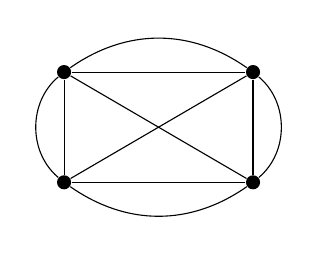
\begin{tikzpicture}[every node/.style={circle,fill,inner sep=1.8pt}]
        \node (A) at (0,1.4) {};
        \node (B) at (2.4,1.4) {};
        \node (C) at (2.4,0) {};
        \node (D) at (0,0) {};
        \draw (A)--(B)--(C)--(D)--(A);
        \draw (A)--(C); \draw (B)--(D);
        \draw (A) to[bend left=35] (B);
        \draw (B) to[bend left=50] (C);
        \draw (C) to[bend left=35] (D);
        \draw (D) to[bend left=50] (A);
    \end{tikzpicture}
    \end{center}
\end{exercise}

\begin{exercise}{10}
    Each of the five platonic solids (tetrahedron, cube, octahedron,
    dodecahedron, icosahedron) has a skeleton graph. For each of these five
    graphs: find a Hamiltonian cycle; determine if it is Eulerian, and if so,
    find an Euler tour.
\end{exercise}

\begin{exercise}{11}
    Let $Q_n$ be the graph whose vertices are all $n$-bit strings, two being
    adjacent iff they differ in exactly one bit.
    \begin{enumerate}[label=(\alph*)]
        \item Draw the cube $Q_3$.
        \item Find a Hamiltonian cycle in $Q_3$.
        \item Describe a method for constructing a Hamiltonian cycle in $Q_n$ for
              each $n$. Think recursively.
        \item Find an Eulerian cycle in $Q_4$.
    \end{enumerate}
\end{exercise}

\begin{exercise}{12}
    Theorem 64 (Euler): \emph{A connected (simple) graph has an Euler tour iff
    every vertex has even degree.} Using Theorem 64 as a black box (don't re-do
    its proof), show that a connected \emph{multigraph} is Eulerian iff every
    vertex has even degree. (Hint: from any multigraph $G$, construct a simple
    graph $H$ such that applying Theorem 64 to $H$ helps.)
\end{exercise}
